\documentclass[12pt,letterpaper]{article}
\usepackage[utf8]{inputenc}
\usepackage[spanish, es-tabla]{babel}
\usepackage[version=3]{mhchem}
\usepackage[journal=jacs]{chemstyle}
\usepackage{amsmath}
\usepackage{amsfonts}
\usepackage{amssymb}
\usepackage{makeidx}
\usepackage{esvect}
\usepackage{xcolor}
\usepackage[stable]{footmisc}
\usepackage[section]{placeins}
%Paquetes necesarios para tablas
\usepackage{longtable}
\usepackage{array}
\usepackage{xtab}
\usepackage{multirow}
\usepackage{colortab}
%Paquete para el manejo de las unidades
\usepackage{siunitx}
\sisetup{mode=text, output-decimal-marker = {,}, per-mode = symbol, qualifier-mode = phrase, qualifier-phrase = { de }, list-units = brackets, range-units = brackets, range-phrase = --}
\DeclareSIUnit[number-unit-product = \;] \atmosphere{atm}
\DeclareSIUnit[number-unit-product = \;] \pound{lb}
\DeclareSIUnit[number-unit-product = \;] \inch{"}
\DeclareSIUnit[number-unit-product = \;] \foot{ft}
\DeclareSIUnit[number-unit-product = \;] \yard{yd}
\DeclareSIUnit[number-unit-product = \;] \mile{mi}
\DeclareSIUnit[number-unit-product = \;] \pint{pt}
\DeclareSIUnit[number-unit-product = \;] \quart{qt}
\DeclareSIUnit[number-unit-product = \;] \flounce{fl-oz}
\DeclareSIUnit[number-unit-product = \;] \ounce{oz}
\DeclareSIUnit[number-unit-product = \;] \degreeFahrenheit{\SIUnitSymbolDegree F}
\DeclareSIUnit[number-unit-product = \;] \degreeRankine{\SIUnitSymbolDegree R}
\DeclareSIUnit[number-unit-product = \;] \usgallon{galón}
\DeclareSIUnit[number-unit-product = \;] \uma{uma}
\DeclareSIUnit[number-unit-product = \;] \ppm{ppm}
\DeclareSIUnit[number-unit-product = \;] \eqg{eq-g}
\DeclareSIUnit[number-unit-product = \;] \normal{\eqg\per\liter\of{solución}}
\DeclareSIUnit[number-unit-product = \;] \molal{\mole\per\kilo\gram\of{solvente}}
\usepackage{cancel}
%Paquetes necesarios para imágenes, pies de página, etc.
\usepackage{graphicx}
\usepackage{lmodern}
\usepackage{fancyhdr}
\usepackage[left=1cm,right=1cm,top=2cm,bottom=3cm]{geometry}

%Instrucción para evitar la indentación
%\setlength\parindent{0pt}
%Paquete para incluir la bibliografía
\usepackage[backend=bibtex,style=chem-acs,biblabel=dot]{biblatex}
\addbibresource{references.bib}

%Formato del título de las secciones

\usepackage{titlesec}
\usepackage{enumitem}
\titleformat*{\section}{\bfseries\large}
\titleformat*{\subsection}{\bfseries\normalsize}

%Creación del ambiente anexos
\usepackage{float}
\floatstyle{plaintop}
\newfloat{anexo}{thp}{anx}
\floatname{anexo}{Anexo}
\restylefloat{anexo}
\restylefloat{figure}

%Modificación del formato de los captions
\usepackage[margin=10pt,labelfont=bf]{caption}

%Paquete para incluir comentarios
\usepackage{todonotes}

%Paquete para incluir hipervínculos
\usepackage[colorlinks=true, 
            linkcolor = blue,
            urlcolor  = blue,
            citecolor = black,
            anchorcolor = blue]{hyperref}

%%%%%%%%%%%%%%%%%%%%%%
%Inicio del documento%
%%%%%%%%%%%%%%%%%%%%%%

\begin{document}
\renewcommand{\labelitemi}{$\checkmark$}

\renewcommand{\CancelColor}{\color{red}}

\newcolumntype{L}[1]{>{\raggedright\let\newline\\\arraybackslash}m{#1}}

\newcolumntype{C}[1]{>{\centering\let\newline\\\arraybackslash}m{#1}}

\newcolumntype{R}[1]{>{\raggedleft\let\newline\\\arraybackslash}m{#1}}

\begin{center}
	\textbf{\LARGE{Práctico 2 - Redes Neuronales 2020}}\\
	\vspace{7mm}
		\textbf{\large{FAMAF - UNC}}\\
	\vspace{4mm}
	\textbf{\large{Alumno: Pablo N. Rosa}}\\
	\textbf{\large{Profesor: Francisco A. Tamarit}}\\
\end{center}

\vspace{4mm}

\section{Introducción}


El modelo neuronal \textbf{integrate-and-fire} es un modelo mono-compartimental que describe la dinámica subumbral del potencial de membrana $V$. La dinámica de disparos está definida por el umbral de disparo ($V_{th}$), es decir, el potencial de membrana a partir del cual la neurona dispara. Después del disparo, $V$ es establecido al potencial de reposo de la neurona. La dinámica subumbral fue inicialmente diseñada para capturar las propiedades pasivas de la membrana, y está dada por la siguiente ecuación diferencial ordinaria de primer orden: 

$$ \dfrac{d V_m(t)}{d t} = \dfrac{1}{\tau_m}(E_L + R_mI_e(t) - V_m(t)) \quad \quad (1)$$

donde $E_L$ es el potencial en reposo, $I_e(t)$ es una corriente eléctrica externa (por convención es positiva) que se inyecta, $R_m$ es la resistencia y $\tau_m$ es el tiempo característico
de la membrana $\tau_m = r_m c_m$ (donde $r_m$ y $c_m$ son respectivamente la resistencia y la capacitancia de la membrana por unidad de área).

Se trabajará con este modelo, usando la ecuación (1) como punto de partida, al analizar su comportamiento con y sin umbral de disparo. Luego se verá cómo influye la forma y magnitud de la corriente externa $I_e$ en la generación de disparos.


\section{Análisis y resultados}

\subsection{Modelo sin umbral}

Resolveremos analíticamente la ecuación (1) sin incorporar el umbral de disparo. Asumiendo que $I_e(t) = I_e$, es decir, una constante e independiente del tiempo. Entonces podemos reescribir (1) como:

$$\dfrac{d V_m(t)}{d t} = \dfrac{1}{\tau_m}(E_L + R_m I_e - V_m(t))$$

Sea $V_{\infty} = E_L + R_m I_e$ (una constante) y definamos una nueva variable $Z(t) = V_{\infty} - V_m(t)$, entonces:  

$$\dfrac{d V_m(t)}{d t} = \dfrac{V_{\infty} - V_m(t)}{\tau_m} = \dfrac{Z(t)}{\tau_m} \hspace{3em} $$

Por otro lado la derivada de $Z(t)$ con respecto a $t$:

$$\dfrac{dZ(t)}{dt} = \dfrac{dV_{\infty}}{dt} - \dfrac{d V_m(t)}{dt} = -\dfrac{d V_m(t)}{dt} = - \dfrac{Z(t)}{\tau_m}$$

Entonces podemos reescribir la ecuacion anterior como:

$$\dfrac{dZ(t)}{Z(t)} = -\dfrac{dt}{\tau_m}$$

e integrando ambos lados como:

$$\int_{Z(0)}^{Z(t)} \frac{dZ'(t)}{Z'(t)} = \ln{\frac{Z(t)}{Z(0)}} = -\frac{1}{\tau_m}\int_{0}^{t} dt' = -\frac{t}{\tau_m}$$

Esto nos da 

$$Z(t) = Z(0)exp\left(- \dfrac{t}{\tau_m}\right) \iff V_{\infty} - V_m(t) = (V_{\infty} - V_m(0))exp\left(- \dfrac{t}{\tau_m}\right)$$

Si $V_m(0) = V_0$, entonces

$$V_m(t) = V_{\infty} - (V_{\infty} - V_0)exp\left(- \dfrac{t}{\tau_m}\right)
$$

$$\iff V_m(t) = E_L + R_m I_e + (V_0 - E_L - R_m I_e)exp\left(- \dfrac{t}{\tau_m}\right) \quad \quad (2)
$$
Con esta expresión para $V_m(t)$, aplicamos una corriente $I_e = 2nA$ constante y con algunos valores de parámetros fijados:

$$V_0 = E_L = -65 mV,\hspace{1em} R_m = 10 M\Omega, \hspace{1em} \tau_m = 10 ms$$

nos queda $$V_m(t) = -45mV + 20mV exp\left(- \dfrac{t}{10ms}\right)$$ 

\begin{figure}[h!]
\begin{floatrow}
\centering
\caption{Solución analítica del modelo sin umbral y corriente constante de 2 nA}
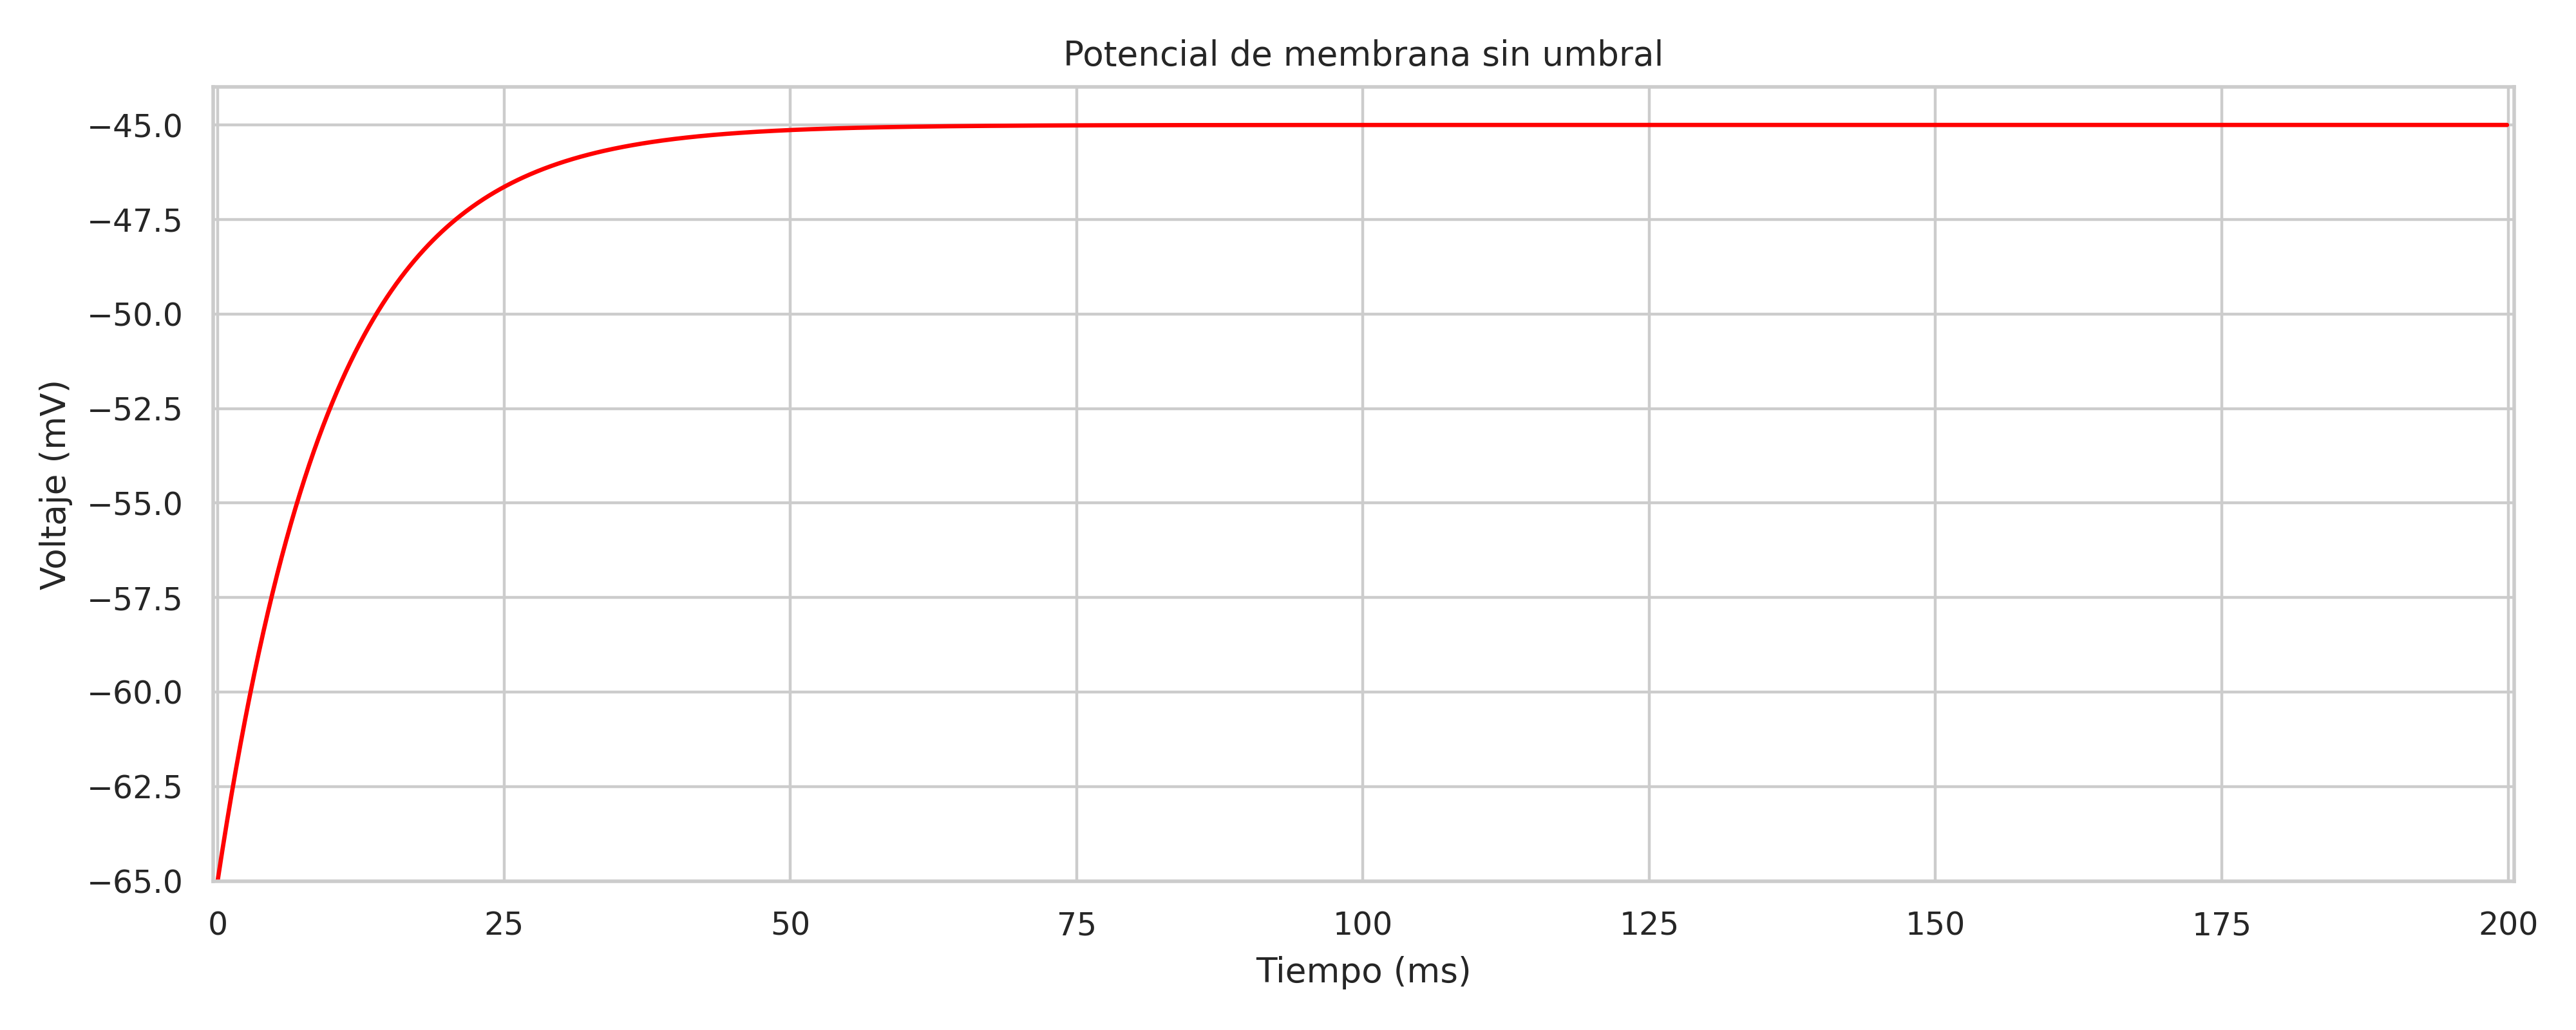
\includegraphics[width=16cm]{../images/sin_umbral.png}
\label{fig:esquema}
\end{floatrow}
\end{figure}


Se observa que si este modelo no incoporara un umbral para el disparo, que resete el potencial de membrana una vez que lo pase, entonces si $t \rightarrow \infty$ el potencial de membrana se quedará en $-45mV$, tal como muestra la Figura 1. Esta ecuación tambien indica que cuando $I_e = 0$, el potencial de membrana se relaja exponencialmente con tiempo contstante $\tau_m$ a $V = E_L$, por lo que $E_L$ es efectivamente el potencial de reposo de la neurona.


\subsection{Modelo con umbral $V_{th}$}

Para generar potenciales de acción, la ecuación inicial (1) se mejora al agregar la regla de que cuando $V_m(t)$ alcance un umbral $V_{th}$, ocurre un disparo y el potencial es reseteado a $V_{reset}$.

Se realizó esto usando el método numérico de Runge Kutta de cuarto orden, con un paso de integración $h = 0.05 s$, los parámetros del inciso anterior y con un umbral de disparos $V_{th} = -50mV$ tal que cuando éste ocurre debe resetearse al valor al potencial de reposo, es decir,  $V_{reset} = E_L$.

\begin{figure}[h!]
\begin{floatrow}
\centering
\caption{Potencial de membrana con umbrales y corriente constante de 2 nA}
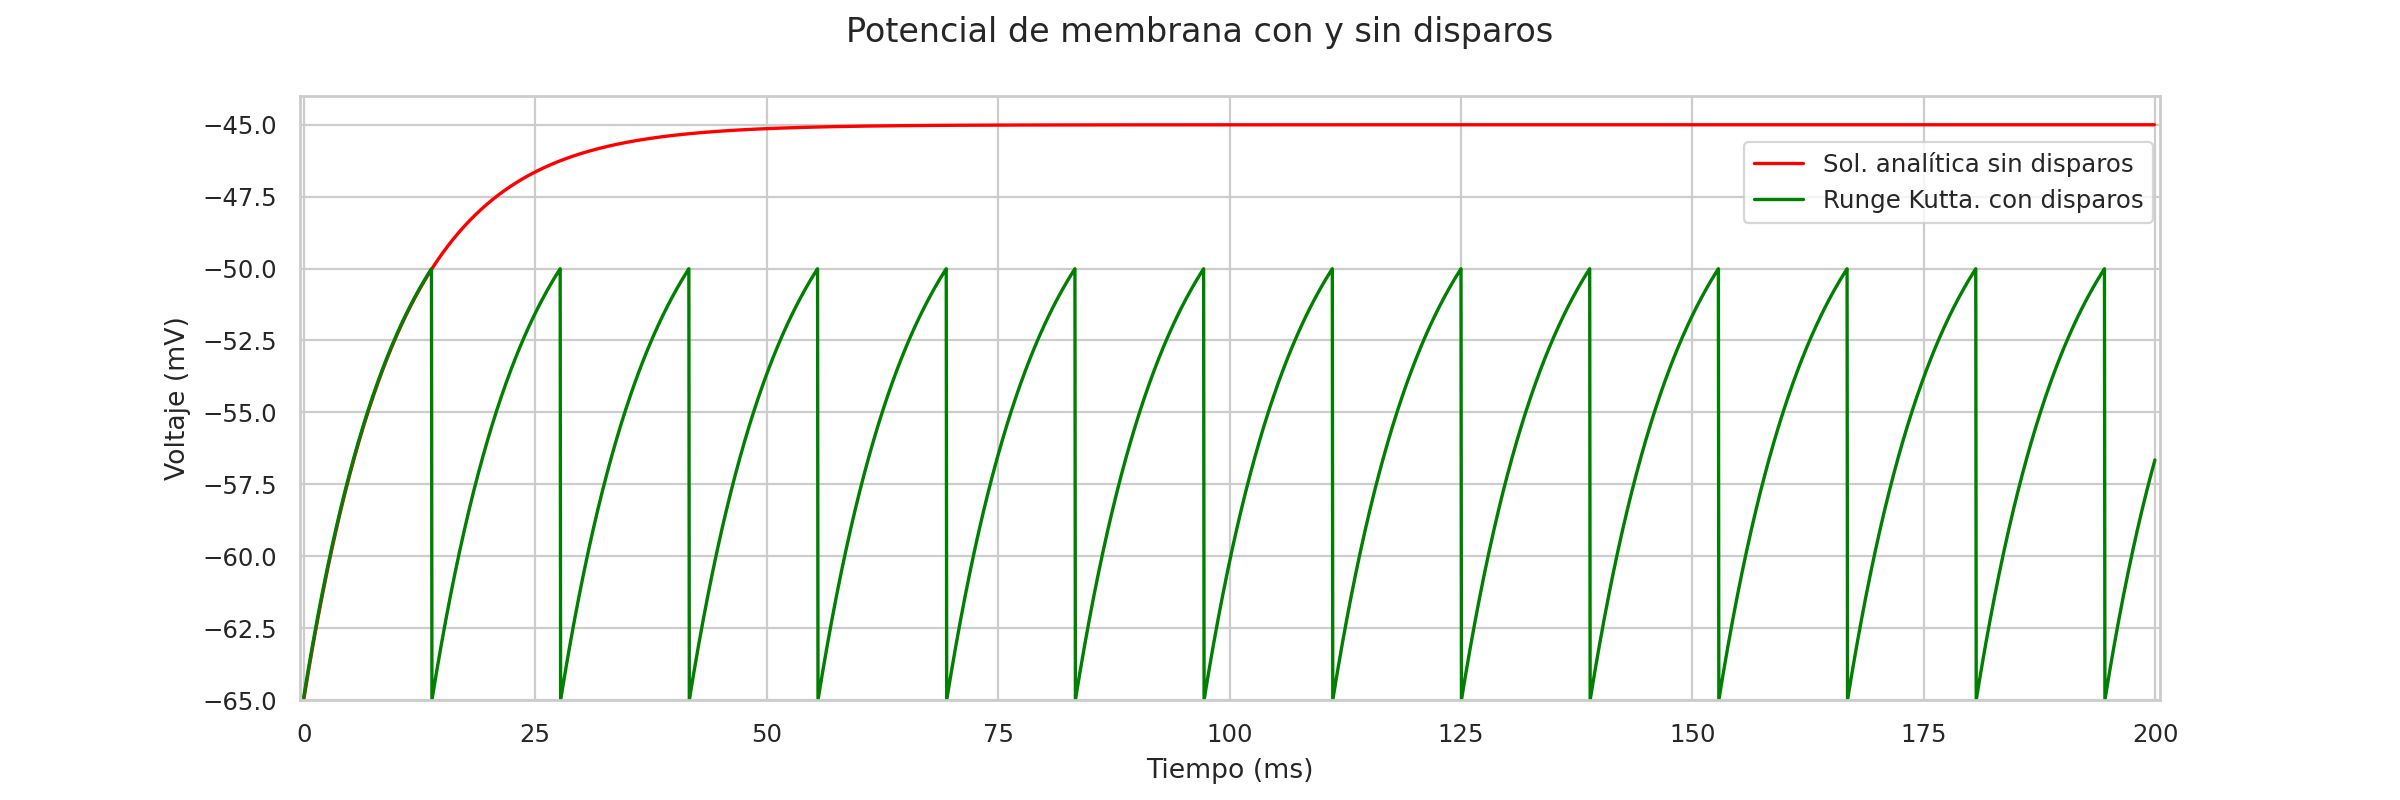
\includegraphics[width=20cm]{../images/con_umbral.png}
\label{fig:esquema}
\end{floatrow}
\end{figure}

La Figura 2 muestra el modelo con y sin disparos. Cuando el potencial llega a los $-50 mV$, ocurre un disparo, y se resetea a $-65mV$. Se observa que con la corriente constante, el patrón de disparos es periódico y ocurre a intervalos regulares. 

La \textit{Frecuencia}, que es la cantidad de disparos por unidad de tiempo, o su inversa, el \textit{Período}, que es el intervalo de tiempo entre dos disparos, también puede ser calculado analíticamente a partir de la ecuacion $(2)$; suponiendo que en el tiempo $t=0s$ la neurona ha disparado, y por ende $V(0) = V_{reset}$, el próximo potencial de acción ocurrirá cuando el potencial de membrana alcance el umbral, es decir, en el tiempo $t=t_{fire}$ donde se cumple:

$$V(t_{fire}) = V_{th} = E_L + R_m I_e + (V_{reset} - E_L - R_m I_e ) exp\left(-\dfrac{t_{fire}}{\tau_m}\right)$$

Despejando el tiempo $t_{fire}$:

$$t_{fire} = \tau_m \ln\left(\dfrac{V_{reset} - E_L - R_mI_e}{V_{th} - E_L - R_m I_e}\right)$$

se obtiene el Período $(\omega)$. Si $I_e$ (la corriente externa medida en $nA$) es una variable independiente entonces el Período $(\omega)$ en función de ella y con los parámetros que se usaron es:

$$\omega(I_e) = 10ms \ln\left(\dfrac{-10I_e}{15 -10I_e }\right)$$

Esta función tiene como dominio todos los valores de $I_e > 1.5 nA$. Los valores negativos no se consideran pues por convención la corriente externa es positiva porque ingresa a la neurona. Por lo tanto, los disparos sólo ocurren con los valores de corrientes mayores a $1.5 nA$. En la Figura 3, se observa la función $\omega(I_e)$ junto con los periodos calculados en simulaciones con corrientes externas en un rango de  $0$ a $6 nA$. 

\begin{figure}[h!]
\begin{floatrow}
\centering
\caption{Períodos de disparos en función de las corrientes externas}
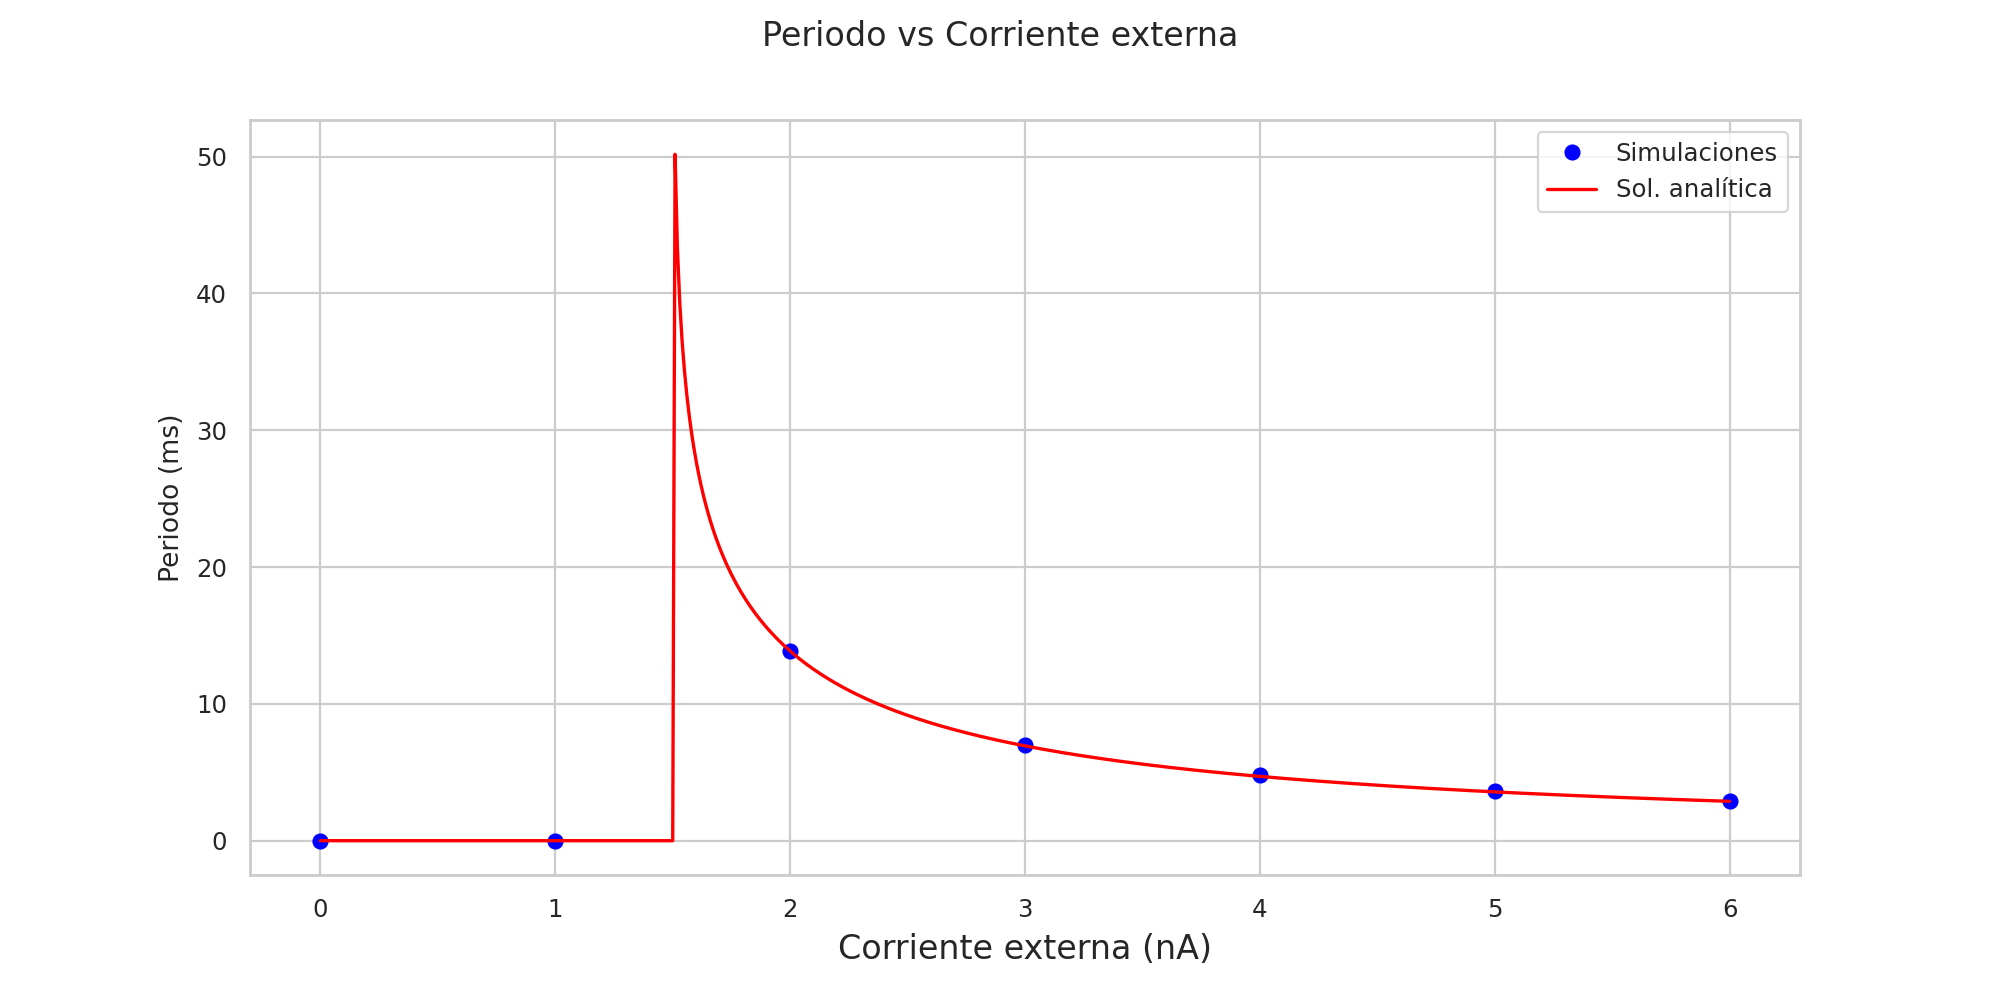
\includegraphics[width=15cm]{../images/periodo_corriente.png}
\label{fig:esquema}
\end{floatrow}
\end{figure}

\subsection{Modelo con una corriente externa variable}

Por último, simularemos un escenario más realista para lo que ocurre con una neurona biológica, con una corriente externa variable que obedece la siguiente ecuación:

$$I_e(t) = 0.35\left(\cos\left({\frac{t}{3}}\right) + \sin\left(\frac{t}{5}\right) + \cos\left(\frac{t}{7}\right) +  
sin\left(\frac{t}{11}\right)+ cos\left(\frac{t}{13}\right)\right)^2
nA$$

La Figura 4 muestra que la neurona dispara cuando llega a $-50mV$, pero no lo hace regularmente como en el caso anterior.

\begin{figure}[h!]
\begin{floatrow}
\centering
\caption{Períodos de disparos en función de las corrientes externas}
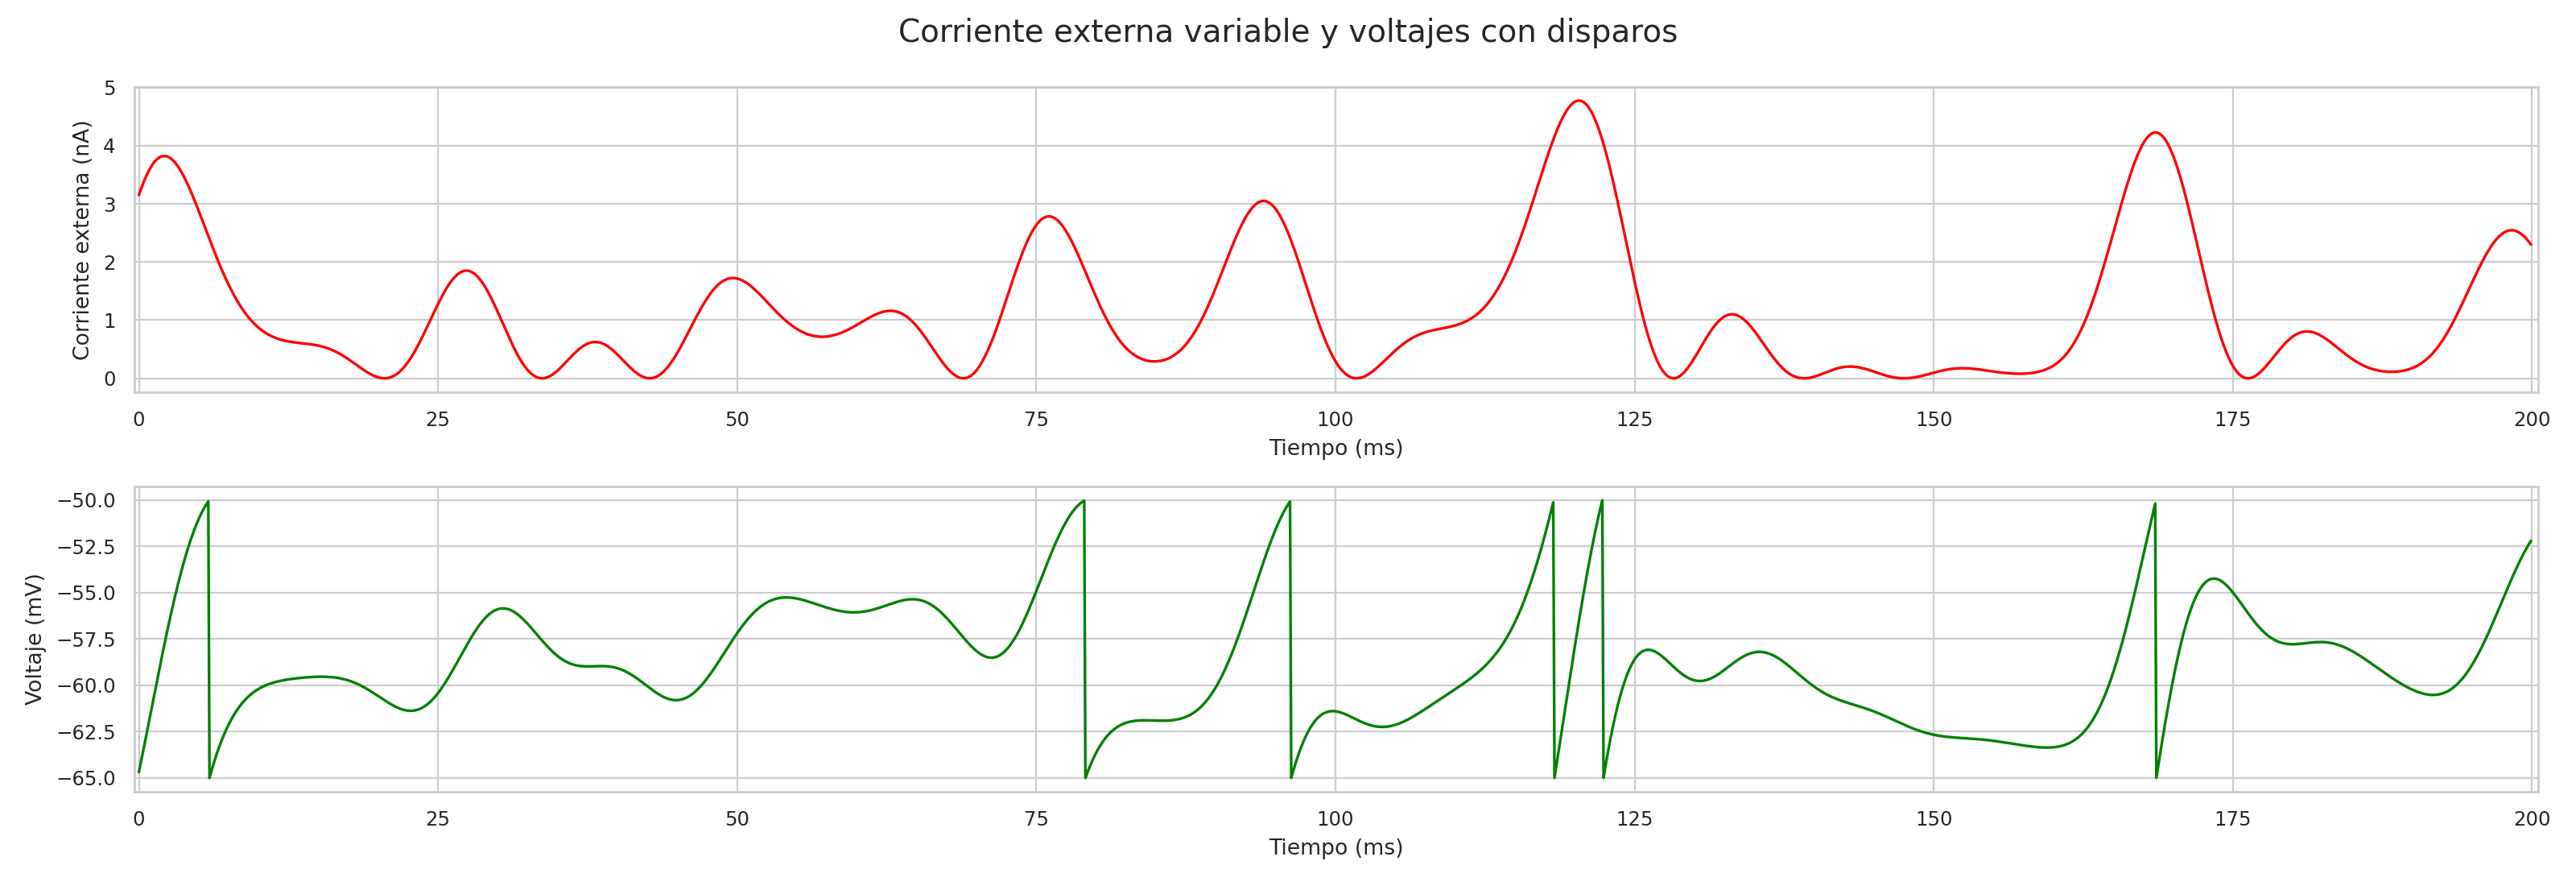
\includegraphics[width=18cm]{../images/no_cte_disparos.png}
\label{fig:esquema}
\end{floatrow}
\end{figure}


\end{document}
